\begin{figure}[H]
\centering
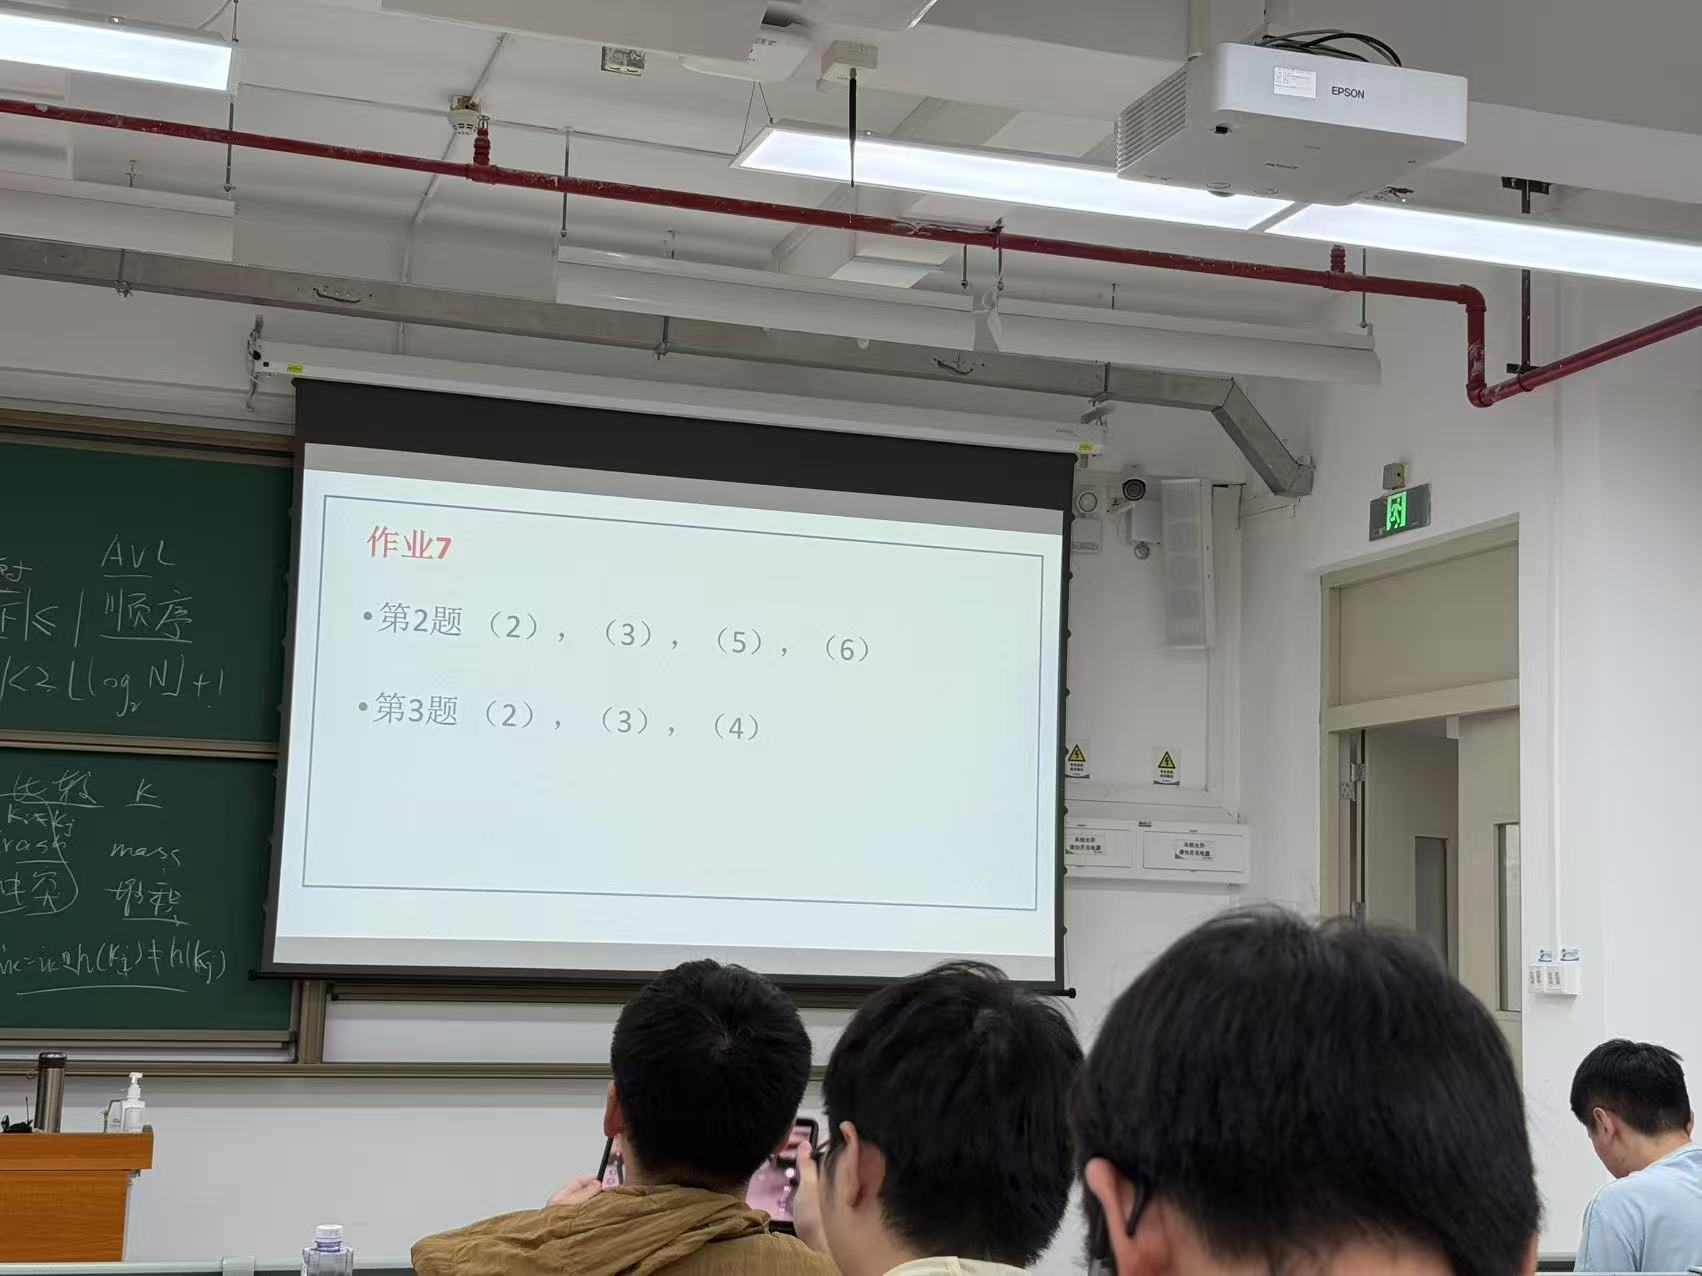
\includegraphics[width=\textwidth]{5978f23fb4375a93ac2f9122776099d5.jpg}
% \caption{}
\label{}
\end{figure}

\begin{exercise}
\begin{figure}[H]
\centering
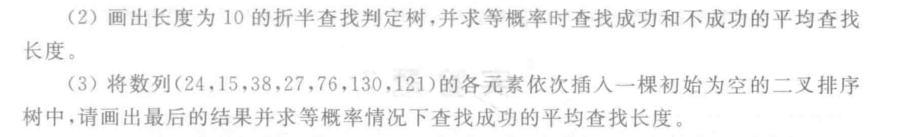
\includegraphics[width=\textwidth]{hw9-2025061723.png}
% \caption{}
\label{}
\end{figure}
\end{exercise}
\begin{figure}[H]
\centering
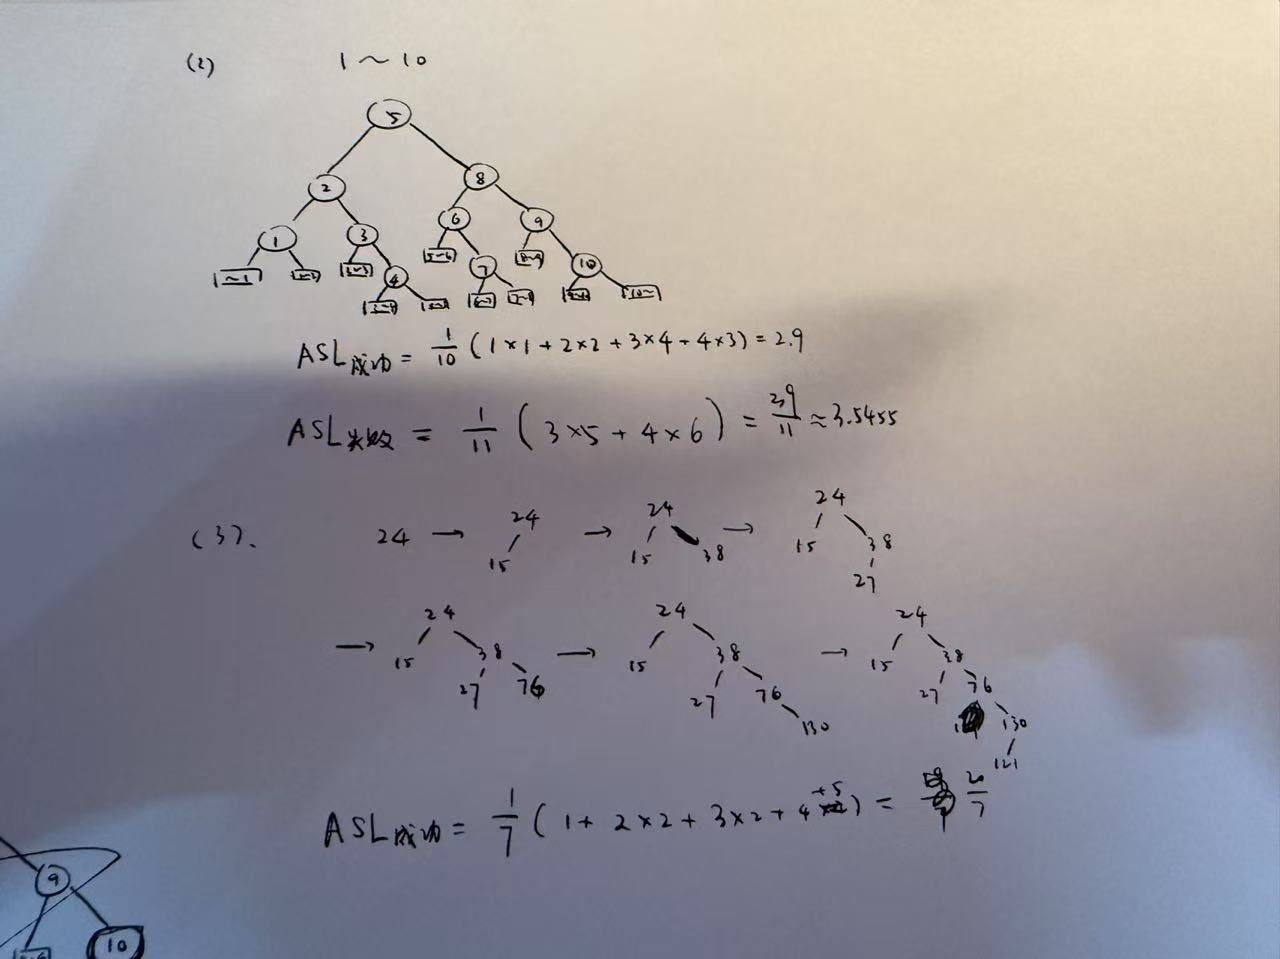
\includegraphics[width=\textwidth]{0e2a5597f75c0f232a6a49431e2831c8.jpg}
% \caption{}
\label{}
\end{figure}

\begin{exercise}
\begin{figure}[H]
\centering
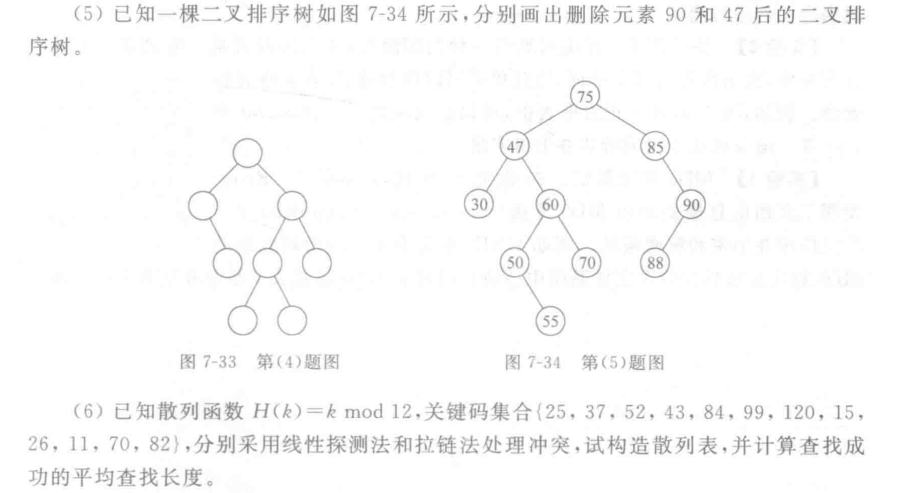
\includegraphics[width=\textwidth]{1-hw9-2025061723.png}
% \caption{}
\label{}
\end{figure}
\end{exercise}
\begin{figure}[H]
\centering
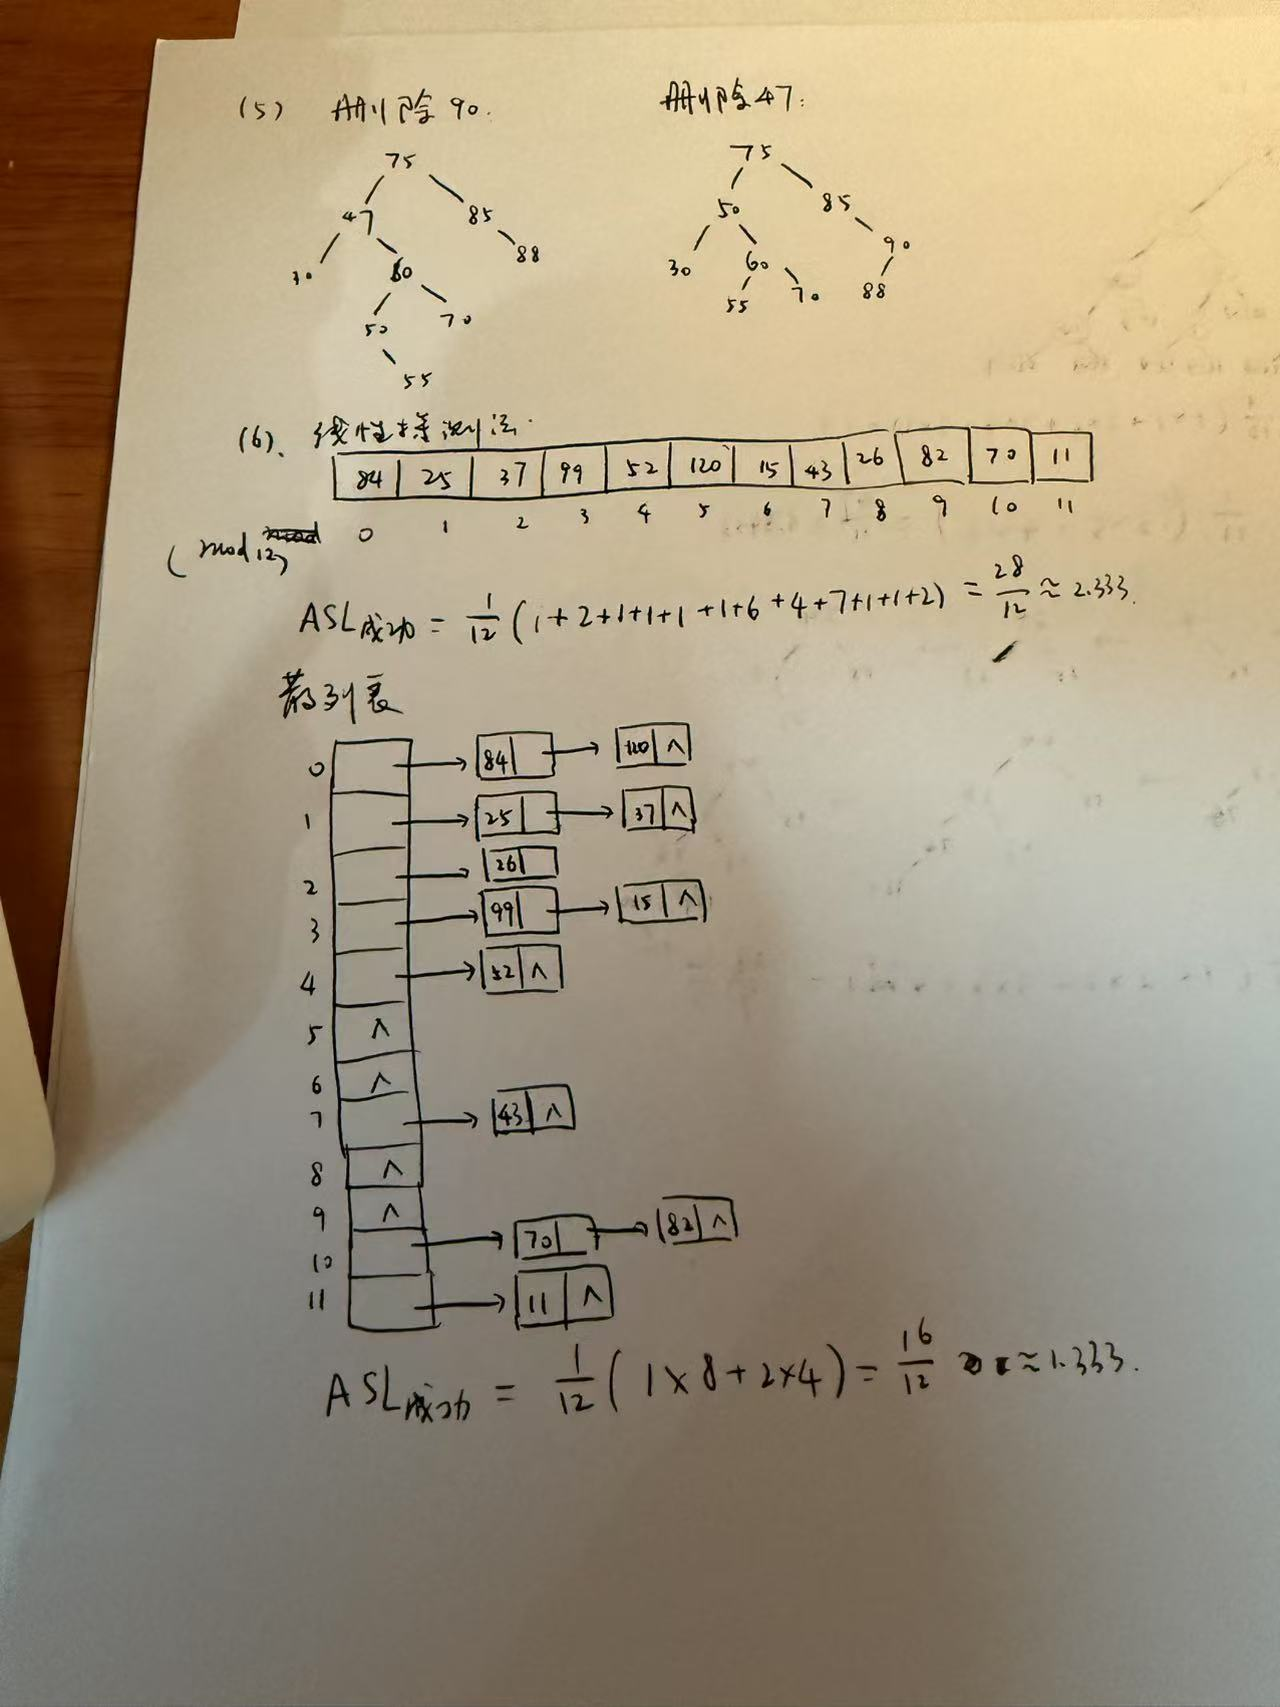
\includegraphics[width=\textwidth]{32aaa76584123e4815d42e6828b02767.jpg}
% \caption{}
\label{}
\end{figure}

\begin{exercise}
\begin{figure}[H]
\centering
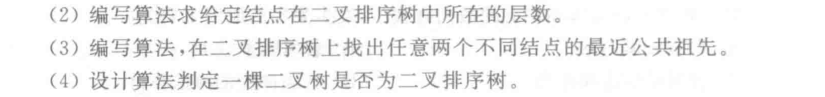
\includegraphics[width=\textwidth]{2-hw9-2025061723.png}
% \caption{}
\label{}
\end{figure}
\end{exercise}
(2)

\begin{lstlisting}
Algorithm GetNodeLevel(root, target)
    Input: root (二叉排序树的根节点), target (目标节点的值)
    Output: level (目标节点所在的层数, 若不存在则返回 -1)

    1. If root is NULL then
           Return -1
       End If

    2. Set currentLevel ← 1
    3. Set currentNode ← root

    4. While currentNode is not NULL do
           If currentNode.value = target then
               Return currentLevel
           Else if target < currentNode.value then
               Set currentNode ← currentNode.left
               Set currentLevel ← currentLevel + 1
           Else
               Set currentNode ← currentNode.right
               Set currentLevel ← currentLevel + 1
           End If
       End While

    5. Return -1  // 目标节点不存在
End Algorithm
\end{lstlisting}
(3)

\begin{lstlisting}
Algorithm FindLowestCommonAncestor(root, p, q)
    Input: root (二叉排序树的根节点), p (第一个节点的值), q (第二个节点的值)
    Output: ancestor (最近公共祖先节点的值, 若不存在则返回 NULL)

    1. If root is NULL then
           Return NULL
       End If

    2. While root is not NULL do
           If root.value > p AND root.value > q then
               Set root ← root.left  // 公共祖先在左子树
           Else if root.value < p AND root.value < q then
               Set root ← root.right  // 公共祖先在右子树
           Else
               Return root.value  // 当前节点是最近公共祖先
           End If
       End While

    3. Return NULL  // 异常情况
End Algorithm
\end{lstlisting}
(4)

\begin{lstlisting}
Algorithm IsBinarySearchTree(root)
    Input: root (二叉树的根节点)
    Output: boolean (true 若为二叉排序树, false 否则)

    // 使用中序遍历检查是否升序
    1. Set prev ← NULL  // 记录前一个访问节点的值

    2. Function InorderCheck(node)
           If node is NULL then
               Return true
           End If

           // 递归检查左子树
           If NOT InorderCheck(node.left) then
               Return false
           End If

           // 检查当前节点是否大于前一个节点
           If prev is not NULL AND node.value <= prev.value then
               Return false
           End If
           Set prev ← node.value

           // 递归检查右子树
           Return InorderCheck(node.right)
       End Function

    3. Return InorderCheck(root)
End Algorithm
\end{lstlisting}